\documentclass[11pt,a4paper]{article}
\usepackage[utf8]{inputenc}
\usepackage[T1]{fontenc}
\usepackage{amsmath, amssymb, graphicx, booktabs, xcolor, tikz}
\IfFileExists{siunitx.sty}{\usepackage{siunitx}}{\providecommand{\SI}[2]{##1\,\ensuremath{\mathrm{##2}}}}
\usetikzlibrary{arrows.meta,positioning,decorations.pathreplacing,calc}
\usepackage[margin=2.5cm]{geometry}
\usepackage[font=small]{caption}
\usepackage[hidelinks]{hyperref}
\graphicspath{{../Images/}}
\allowdisplaybreaks

% Draft marker: redefine as \newcommand{\todo}[1]{} for the final version
\newcommand{\todo}[1]{\textcolor{red}{[TODO: #1]}}
\newcommand{\code}[1]{\texttt{\small #1}}

\title{First Report\\[0.5em]
  \large VTOL Technical Report \textit{Versatile}}
\author{Álvaro Martínez Blanco\\ \small Universidad de Sevilla}
\date{\today}

\begin{document}
\maketitle

\begin{abstract}
This report documents the current state of PATRONUS, a MATLAB/CasADi framework for
trajectory optimisation of a four-engine tilt-rotor UAV. It covers the 3-DOF longitudinal
model, the take-off optimal control problem, the flatness-based initial guess, the direct
collocation transcription (trapezoidal and Hermite--Simpson) and its solution with IPOPT.
The take-off from hover to a trimmed hover at \SI{30}{m} converges with the full nonlinear
aerodynamic and propulsive models. Known model limitations and the planned research
lines (singular arcs, differential flatness, successive convexification, indirect methods
and the hover-to-cruise transition) close the report.
\end{abstract}

\tableofcontents
\newpage

% =====================================================================
\section{Equations of motion and models}\label{sec:models}

\subsection{Hypotheses}
\begin{itemize}
  \item Rigid aircraft, 3-DOF longitudinal motion (surge, heave, pitch), flat non-rotating
        Earth, standard constant density $\rho = \SI{1.2133}{kg/m^3}$, no wind.
  \item Two tilting rotor groups ($i=1$ front at the wing, $i=2$ rear at the tail), each of
        $N_e = 2$ engines, with tilt $\epsilon_i$ and speed $n_i$ as controls.
        The elevator is not modelled in the tail yet.
  \item Quasi-steady aerodynamics and propeller maps; no rotor--wing interference other than
        the tail downwash $\xi(\alpha)$ and the nacelle drag in the rotor slipstream.
  \item Rotor in-plane force $H_i = 0$ (\code{CH\_version = 'zeros'}).
  \item Forward flight only ($u_b \ge 0$), so $|\alpha| < 90^\circ$.
\end{itemize}

\subsection{Equations of motion}\label{sec:eom}
The state is $\mathbf{x} = (x, h, v_x, v_h, \theta, q, E)$ and the control
$\mathbf{u} = (\epsilon_1, \epsilon_2, n_1, n_2)$. The translational equations are written in
\emph{inertial axes} ($x$ forward, $h$ up):
\begin{equation}
\dot x = v_x, \quad \dot h = v_h, \quad
\dot v_x = \frac{F_x}{m}, \quad \dot v_h = \frac{F_h}{m}, \quad
\dot\theta = q, \quad \dot q = \frac{M}{I_{yy}}, \quad
\dot E = \frac{P_1 + P_2}{\eta}.
\label{eq:eom}
\end{equation}
$E$ is the electrical energy drawn from the battery. The wind quantities are derived from
the states (Figure~\ref{fig:angles}) with an airspeed regularisation $V_\varepsilon = \SI{0.5}{m/s}$:
\begin{gather}
V = \sqrt{v_x^2 + v_h^2 + V_\varepsilon^2}, \qquad
u_b = v_x\cos\theta + v_h\sin\theta, \qquad w_b = v_x\sin\theta - v_h\cos\theta, \\
\alpha = \operatorname{atan2}\!\big(w_b,\ \sqrt{u_b^2 + V_\varepsilon^2}\big), \qquad
\gamma = \theta - \alpha .
\end{gather}
The resultant forces and moment are
\begin{align}
F_x &= -D_a\cos\gamma - L_a\sin\gamma
 + \textstyle\sum_i \big[ T_i\cos(\theta+\epsilon_i) - D_{n,i}\cos(\theta+\epsilon_i-\alpha_{n,i}) \big], \\
F_h &= -D_a\sin\gamma + L_a\cos\gamma
 + \textstyle\sum_i \big[ T_i\sin(\theta+\epsilon_i) - D_{n,i}\sin(\theta+\epsilon_i-\alpha_{n,i}) \big] - m g, \\
M &= M_{\text{aero}} + M_{E,1} + M_{E,2} + M_{n,1} + M_{n,2},
\end{align}
with lift and drag summed over wing, fuselage and tail. The full moment build-up is given in
Appendix~\ref{app:model}.


\begin{figure}[h]
\centering
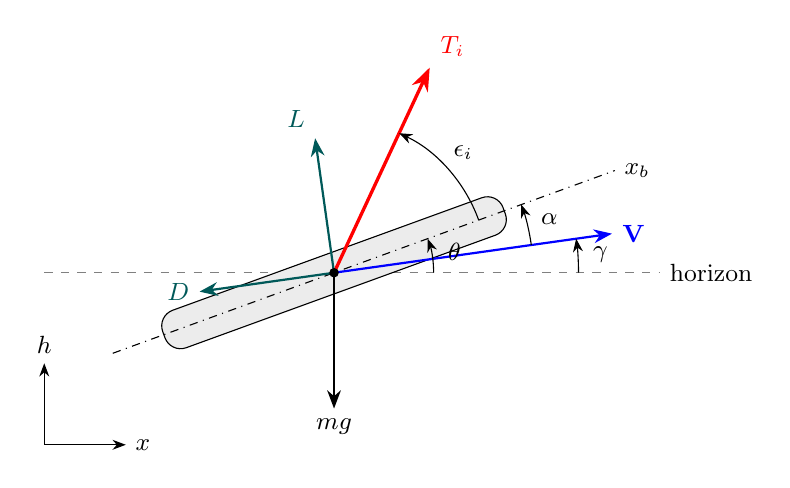
\begin{tikzpicture}[>=Stealth, scale=1.15, font=\small]
  % inertial axes
  \draw[->] (-3.2,-1.9) -- (-2.3,-1.9) node[right]{$x$};
  \draw[->] (-3.2,-1.9) -- (-3.2,-1.0) node[above]{$h$};
  % horizon
  \draw[dashed, gray] (-3.2,0) -- (3.6,0) node[right, black]{horizon};
  % body
  \begin{scope}[rotate=20]
    \draw[fill=gray!15, rounded corners=6pt] (-2,-0.22) rectangle (2,0.22);
    \draw[dashdotted] (-2.6,0) -- (3.3,0) node[right]{$x_b$};
  \end{scope}
  % forces and velocity
  \draw[->, thick, blue] (0,0) -- (8:3.1) node[right]{$\mathbf{V}$};
  \draw[->, very thick, red] (0,0) -- (65:2.5) node[above right]{$T_i$};
  \draw[->, thick, teal!70!black] (0,0) -- (98:1.5) node[above left]{$L$};
  \draw[->, thick, teal!70!black] (0,0) -- (188:1.5) node[left]{$D$};
  \draw[->, thick] (0,0) -- (0,-1.5) node[below]{$mg$};
  % angles
  \draw[->] (0:1.1) arc (0:20:1.1);   \node at (10:1.35) {$\theta$};
  \draw[->] (0:2.7) arc (0:8:2.7);    \node at (4:2.95) {$\gamma$};
  \draw[->] (8:2.2) arc (8:20:2.2);   \node at (14:2.45) {$\alpha$};
  \draw[->] (20:1.7) arc (20:65:1.7); \node at (43:1.95) {$\epsilon_i$};
  \fill (0,0) circle (1.5pt);
\end{tikzpicture}
\caption{Angle and force conventions in the longitudinal plane. $\theta$ is measured from the
horizon to the body axis, $\gamma$ to the velocity, so $\alpha = \theta - \gamma$. The thrust acts
at $\theta + \epsilon_i$ from the horizon and the propeller inflow angle is $\phi_i = \alpha + \epsilon_i$.
Lift is normal and drag parallel to $\mathbf{V}$. In a vertical climb $\gamma = 90^\circ$ and
$\alpha \to -90^\circ$.}
\label{fig:angles}
\end{figure}

\paragraph{Decision: inertial axes.} Wind axes are undefined in hover ($V=0$) and body axes
add the $qw$, $qu$ coupling terms. Inertial axes keep the translational equations linear in
the forces and well defined from hover to forward flight. The cost is that $\alpha$ and
$\gamma$ become derived quantities, which is why $V_\varepsilon$ is needed.

\paragraph{Decision: regularisation.} $V \ge V_\varepsilon > 0$ keeps $\cos\gamma$, $\sin\gamma$,
$J_i$ and $\alpha$ smooth at hover. Every non-smooth function in the model is replaced by a
smooth one ($|x| \to \sqrt{x^2+10^{-6}}$) so that IPOPT sees $C^2$ functions.

\subsection{Aerodynamic model}\label{sec:aero}
With $\bar q = \tfrac12\rho V^2$, each surface $s \in \{w, f, t\}$ contributes
$L_s = \bar q S_s C_{L,s}$, $D_s = \bar q S_s C_{D,s}$, and a pure moment
$\bar q S_s \ell_s C_{M,s}$. The tail sees $\alpha - \xi$, with linear downwash
$\xi = 0.01 + 0.3\,\alpha$, and its forces are rotated by $\xi$ back to freestream axes.

The coefficients $C_{L,s}$, $C_{D,s}$, $C_{M,s}$ are tabulated over
$\alpha \in [-180^\circ, 180^\circ]$ every $10^\circ$ and interpolated with cubic B-splines
(CasADi \code{interpolant}), see Figure~\ref{fig:aero}.

\paragraph{Decision: full-envelope tables.} During take-off $\alpha$ reaches $-90^\circ$ (vertical
climb), so the usual linear-plus-quadratic polar is not valid. A cubic B-spline gives a $C^2$
model over the whole range. The coarse $10^\circ$ grid smooths the stall region, which is
acceptable for a first take-off study but not for the cruise-transition corridor.

\begin{figure}[h]
  \centering
  \includegraphics[width=0.32\textwidth]{Aero_Curves_Wing.pdf}\hfill
  \includegraphics[width=0.32\textwidth]{Aero_Curves_Fus.pdf}\hfill
  \includegraphics[width=0.32\textwidth]{Aero_Curves_Tail.pdf}
  \caption{Wing, fuselage and tail aerodynamic coefficients.}
  \label{fig:aero}
\end{figure}

\subsection{Propulsive model}\label{sec:prop}
Each rotor group sees the advance ratio and inflow angle
\begin{equation}
J_i = \frac{V}{n_i D}, \qquad \phi_i = \alpha + \epsilon_i,
\end{equation}
and produces
\begin{equation}
T_i = N_e\, \rho n_i^2 D^4\, C_T(J_i,\phi_i), \qquad
P_i = N_e\, \rho n_i^3 D^5\, C_P(J_i,\phi_i).
\end{equation}
$C_T$ and $C_P$ are polynomial fits of degree 4 in $J$ and 3 in $|\phi|$ (Figure~\ref{fig:prop}):
\begin{equation}
C(J,\phi) = a_1 + b_1 J + c_1 J^2 + d_1 J^3 + e_1 J^4
 + |\phi|(b_2 J + c_2 J^2 + d_2 J^3) + |\phi|^2 (b_3 J + c_3 J^2) + |\phi|^3 b_4 J .
\end{equation}
\todo{source of the fits (wind-tunnel data, propeller reference), fitting range}

\paragraph{Decision: $C_P$-based power.} The shaft power is computed from $C_P$, not from
$P = TV$. The latter vanishes in hover, which is where the take-off spends most of its
energy. $P = TV$ was only used while debugging the cruise problem.

\paragraph{Nacelle drag.} The induced velocity $v_i$ of each rotor solves the momentum-theory quartic
\begin{equation}
v_i^4 + 2\sin\phi_i\, V v_i^3 + V^2 v_i^2 - K_i^2 = 0, \qquad K_i = \frac{T_i}{\tfrac12\rho D^2},
\end{equation}
by 8 fixed Newton iterations started from the hover solution $\sqrt{K_i}$. The nacelle then sees the
local flow angle $\alpha_{n,i}$ and dynamic pressure of the slipstream (Appendix~\ref{app:model}).
A fixed number of iterations keeps the expression explicit and differentiable by CasADi.

\begin{figure}[h]
  \centering
  \includegraphics[width=0.8\textwidth]{Prop_Maps.pdf}
  \caption{Propeller maps $C_T(J,\phi)$ and $C_P(J,\phi)$.}
  \label{fig:prop}
\end{figure}

\subsection{Battery model (Shepherd)}\label{sec:battery}
In the current take-off problem the battery is an ideal energy store: $E$ integrates the bus power
and the objective is $E(t_f)/E_\text{batt}$, with $E_\text{batt} = \SI{2.16}{MJ}$
(\SI{3}{kg} at \SI{720}{kJ/kg}). The Shepherd model, already implemented in a separate battery
discharge simulation, is the next step. In Tremblay's form of Shepherd's equation the terminal
voltage is
\begin{equation}
V_b = E_0 - K\frac{Q}{Q - it}\, i - R\, i + A\, e^{-B\, it},
\end{equation}
with $it = \int_0^t i\,d\tau$ the extracted charge, $Q$ the capacity, $R$ the internal resistance,
$K$ the polarisation constant, and $A$, $B$ the exponential-zone parameters. Coupled to the
trajectory, the bus power balance $V_b(it, i)\, i = (P_1 + P_2)/\eta$ fixes the current, and the state
$E$ is replaced by the extracted charge $it$.
\todo{parameters and cell data; check the form against the existing battery script}

\paragraph{Decision: Shepherd.} It needs few parameters, is smooth in the operating range and
captures the voltage sag at high current, which matters in hover-dominated segments. Equivalent
circuit models add transient states with time constants far shorter than the manoeuvre.

\subsection{Aircraft data}
\begin{table}[h]
\centering\small
\begin{tabular}{@{}llll@{}}
\toprule
Mass $m$ & \SI{25.54}{kg} \todo{CAD check} & Pitch inertia $I_{yy}$ & \SI{98.19}{kg\,m^2} \\
Wing / tail area & \SI{0.48186}{m^2} each & Fuselage area, length & \SI{0.4094}{m^2}, \SI{1.75}{m} \\
Propeller diameter $D$ & \SI{0.718}{m} & Engines per group $N_e$ & 2 \\
Max thrust per engine & \SI{238.4}{N} & Max power per engine & \SI{6.7}{kW} \\
Max speed $n_\text{max}$ & \SI{78.125}{rps} & Propulsive efficiency $\eta$ & 0.8192 \\
\bottomrule
\end{tabular}
\caption{2Wings aircraft data (\code{cruise\_config}).}
\end{table}

% =====================================================================
\section{Problem formulation}\label{sec:formulation}

The take-off is posed as a free-final-time Bolza problem:
\begin{equation}
\begin{aligned}
\min_{\mathbf{u}(\cdot),\, t_f} \quad & J = \Phi\big(\mathbf{x}(t_f), t_f\big) \\
\text{s.t.} \quad & \dot{\mathbf{x}} = f(\mathbf{x},\mathbf{u}), \\
& \mathbf{g}(\mathbf{x},\mathbf{u}) \le 0, \quad
  \mathbf{x}_\text{min} \le \mathbf{x} \le \mathbf{x}_\text{max}, \quad
  \mathbf{u}_\text{min} \le \mathbf{u} \le \mathbf{u}_\text{max}, \quad |\dot{\mathbf{u}}| \le \dot{\mathbf{u}}_\text{max}, \\
& \mathbf{x}(0) = \mathbf{x}_0, \quad \boldsymbol\psi\big(\mathbf{x}(t_f), \dot{\mathbf{x}}(t_f)\big) = 0 .
\end{aligned}
\end{equation}

\subsection{Objective function}
Two objectives are registered:
\begin{equation}
J_E = 100\,\frac{E(t_f)}{E_\text{batt}} \;[\%], \qquad
J_t = \frac{t_f}{t_\text{ref}}, \quad t_\text{ref} = \SI{10}{s}.
\end{equation}
Both are $O(1)$ by construction. A control-rate regulariser is added to either of them:
\begin{equation}
R = w \sum_{j} \int_0^1 \left(\frac{d\tilde u_j}{d\tau}\right)^2 d\tau, \qquad w = 10^{-3},
\end{equation}
with $\tilde u_j$ the scaled controls and $\tau = t/t_f$.

\paragraph{Decision: regulariser.} Four controls act on three translational and rotational
degrees of freedom, so the problem has flat directions (tilt and speed can trade the same pitching moment).
The regulariser removes them and the chattering they cause, at the price of slightly
rounding bang-bang arcs. Being an integral in $\tau$, its weight does not depend on $N$ or on the scheme.

\subsection{Path constraints}
At every node, normalised by their limits so that all multipliers are comparable:
\begin{gather}
C_{T,i} \ge 0, \quad C_{P,i} \ge 0, \quad
T_i \le N_e T_\text{max}, \quad P_i \le N_e P_\text{max}, \quad
J_i \le 1.2, \quad |\phi_i| \le 90^\circ .
\end{gather}
The last two keep the propeller fits inside their data range.
Actuator rates are limited to $|\dot\epsilon_i| \le \SI{45}{deg/s}$ and $|\dot n_i| \le \SI{50}{rps/s}$
\todo{placeholder values, check servo and motor datasheets}.

\subsection{Bounds and boundary conditions}
\begin{table}[h]
\centering\small
\begin{tabular}{@{}lccccc@{}}
\toprule
Variable & Min & Max & $t=0$ & $t=t_f$ & Note \\
\midrule
$x$ [m]          & 0     & 200 & 0 & free & $x(t_f) \le \SI{2}{m}$ \\
$h$ [m]          & 0     & 36  & 0 & 30   & \\
$v_x$ [m/s]      & 0     & 30  & 0 & 0    & $\dot v_x(t_f) = 0$ \\
$v_h$ [m/s]      & $-5$  & 10  & 0 & 0    & $\dot v_h(t_f) = 0$ \\
$\theta$ [deg]   & $-20$ & 20  & 0 & 0    & \\
$q$ [rad/s]      & $-0.6$& 0.6 & 0 & 0    & $\dot q(t_f) = 0$ \\
$E$ [MJ]         & 0     & 2.16& 0 & free & \\
\midrule
$\epsilon_i$ [deg] & 0 & 110 & \multicolumn{2}{c}{--} & rate limited \\
$n_i$ [rps]        & 10 & 78.125 & \multicolumn{2}{c}{--} & rate limited \\
$t_f$ [s]          & 2 & 60 & \multicolumn{2}{c}{--} & free \\
\bottomrule
\end{tabular}
\caption{Bounds and boundary conditions of the take-off (\code{vtol\_config}).}
\end{table}

\paragraph{Decision: terminal trim.} $v_x = v_h = q = 0$ at $t_f$ only says that the aircraft is
momentarily at rest. Adding $\dot v_x = \dot v_h = \dot q = 0$ forces a trimmed hover, with forces and
pitching moment balanced, so the take-off can be chained to the next segment.

% =====================================================================
\section{Initial guess generation}\label{sec:guess}

IPOPT converges to a local optimum near its starting point, so the guess decides both
convergence and which solution is found. The guess is built from the differential flatness of
the simplified model (Appendix~\ref{app:flatness}):
\begin{enumerate}
  \item \textbf{Flat outputs.} $x(t)$, $h(t)$ and $\theta(t)$ are quintic polynomials matching
        position, velocity and zero acceleration at both ends, with $x(t_f) = x_\text{TO}$.
  \item \textbf{States by differentiation.} $v_x = \dot x$, $v_h = \dot h$, $q = \dot\theta$.
  \item \textbf{Controls by inversion.} The required thrust vector follows from the force balance,
        \begin{equation}
        \mathbf{T} = m\big(\ddot x,\ \ddot h + g\big) - \mathbf{F}_\text{aero}(v_x, v_h, \theta),
        \qquad \epsilon = \operatorname{atan2}(T_h, T_x) - \theta,
        \end{equation}
        assuming $\epsilon_1 = \epsilon_2$, $H = 0$ and no nacelle drag. The split $T_1/T_2$ trims the
        pitching moment $I_{yy}\ddot\theta - M_\text{aero}$ (equal split when $|\sin\epsilon| < 0.2$),
        and $n_i$ follows from $T_i$ by fixed-point iteration on $C_T(J(n_i), \phi_i)$.
  \item \textbf{Energy.} $E(t)$ is the cumulative integral of $(P_1+P_2)/\eta$ with the inverted controls.
  \item \textbf{Duration sweep.} The guess is built for $t_f \in \{5, 10, 15\}\,$s and checked against
        bounds, boundary conditions, path constraints and the dynamics residual (tolerance 5\%).
        The feasible candidate with the lowest objective is kept; otherwise the least infeasible one.
\end{enumerate}

\paragraph{Decision: flatness instead of interpolation.} A linear interpolation between the
boundary conditions is not dynamically consistent: the controls do not produce the guessed
accelerations, and IPOPT starts with large defects and usually enters restoration. The flat guess
satisfies the simplified dynamics exactly, so the starting infeasibility only comes from the terms it
neglects.

% =====================================================================
\section{Transcription, collocation and CasADi}\label{sec:transcription}

\subsection{Direct transcription}
The time is normalised, $t = \tau t_f$ with $\tau \in [0,1]$, on a uniform grid of $N = 40$
intervals, $h = t_f/N$. The NLP decision vector is
\begin{equation}
\mathbf{w} = \big[\mathbf{x}_0, \dots, \mathbf{x}_N,\ \mathbf{u}_0, \dots, \mathbf{u}_N,\
(\mathbf{u}_{1/2}, \dots, \mathbf{u}_{N-1/2}),\ t_f \big],
\end{equation}
with midpoint controls only for Hermite--Simpson. The ODE becomes the defect equalities of the
chosen scheme; path constraints are imposed at every node (Figure~\ref{fig:grid}).


\begin{figure}[h]
\centering
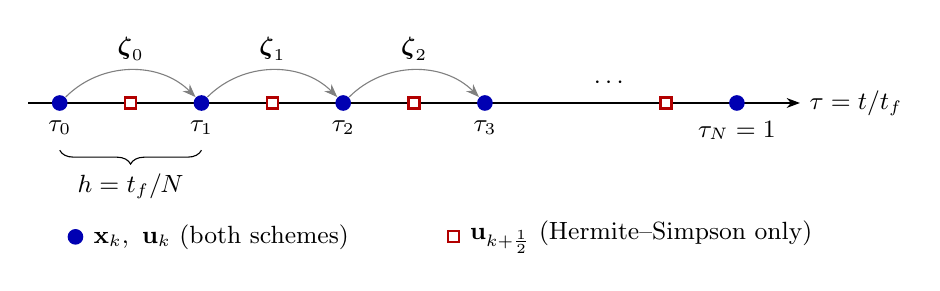
\begin{tikzpicture}[>=Stealth, font=\small,
  node/.style={circle, fill=blue!70!black, inner sep=2pt},
  mid/.style={rectangle, draw=red!70!black, fill=white, thick, inner sep=2pt}]
  \draw[->] (-0.4,0) -- (9.4,0) node[right]{$\tau = t/t_f$};
  \foreach \i/\lab in {0/0, 1/1, 2/2, 3/3} {
    \node[node] (n\i) at (1.8*\i,0) {};
    \node[below=3pt] at (1.8*\i,0) {$\tau_{\lab}$};
  }
  \node[node] (nN) at (8.6,0) {};
  \node[below=3pt] at (8.6,0) {$\tau_N = 1$};
  \node at (7.0,0.25) {$\cdots$};
  \foreach \i in {0,1,2} { \node[mid] at (1.8*\i+0.9,0) {}; }
  \node[mid] at (8.6-0.9,0) {};
  % defects
  \foreach \i/\j in {0/1, 1/2, 2/3} {
    \draw[->, gray, bend left=45] (n\i) to node[above, black]{$\boldsymbol\zeta_{\i}$} (n\j);
  }
  % h brace
  \draw[decorate, decoration={brace, mirror, amplitude=5pt}] (0,-0.6) -- (1.8,-0.6)
    node[midway, below=5pt]{$h = t_f/N$};
  % legend
  \node[node, label=right:{$\mathbf{x}_k,\ \mathbf{u}_k$ (both schemes)}] at (0.2,-1.7) {};
  \node[mid, label=right:{$\mathbf{u}_{k+\frac12}$ (Hermite--Simpson only)}] at (5.0,-1.7) {};
\end{tikzpicture}
\caption{Collocation grid. States and controls live at the $N+1$ nodes; Hermite--Simpson adds
a control at each interval midpoint. Each interval contributes one defect $\boldsymbol\zeta_k = 0$
linking consecutive states, and $t_f$ is a single extra decision variable.}
\label{fig:grid}
\end{figure}

\paragraph{Decision: direct rather than indirect.} Direct collocation needs no costate guess,
handles path and control constraints as ordinary NLP constraints, and has a large basin of
convergence. The indirect method is more accurate but would require the switching structure of the
solution in advance (Section~\ref{sec:future}).

\subsection{Collocation schemes}
\begin{align}
\text{Trapezoidal (order 2):}\quad & \mathbf{x}_{k+1} - \mathbf{x}_k - \tfrac{h}{2}\big(\mathbf{f}_k + \mathbf{f}_{k+1}\big) = 0, \\
\text{Hermite--Simpson (order 4):}\quad & \mathbf{x}_{k+1} - \mathbf{x}_k - \tfrac{h}{6}\big(\mathbf{f}_k + 4\mathbf{f}_{k+\frac12} + \mathbf{f}_{k+1}\big) = 0, \\
& \mathbf{x}_{k+\frac12} = \tfrac12(\mathbf{x}_k + \mathbf{x}_{k+1}) + \tfrac{h}{8}(\mathbf{f}_k - \mathbf{f}_{k+1}),
\end{align}
with $\mathbf{f}_{k+\frac12} = f(\mathbf{x}_{k+\frac12}, \mathbf{u}_{k+\frac12})$
(compressed form: the midpoint state is not a decision variable). Figure~\ref{fig:quad} shows both schemes as quadrature rules.


\begin{figure}[h]
\centering
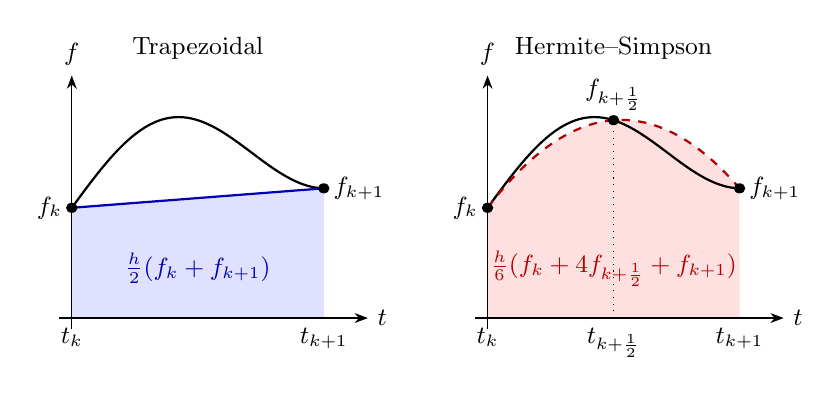
\begin{tikzpicture}[>=Stealth, font=\small, xscale=1.6, yscale=1.4]
  % ----- trapezoidal -----
  \begin{scope}
    \fill[blue!12] (0,0) -- (0,1.0) -- (2,1.1766) -- (2,0) -- cycle;
    \draw[->] (-0.1,0) -- (2.35,0) node[right]{$t$};
    \draw[->] (0,-0.1) -- (0,2.2) node[above]{$f$};
    \draw[thick, domain=0:2, samples=60] plot (\x, {1.0+0.35*\x+0.55*sin(2.2*\x r)});
    \draw[blue!70!black, thick] (0,1.0) -- (2,1.1766);
    \fill (0,1.0) circle (1.3pt) node[left]{$f_k$};
    \fill (2,1.1766) circle (1.3pt) node[right]{$f_{k+1}$};
    \node[below] at (0,0) {$t_k$};  \node[below] at (2,0) {$t_{k+1}$};
    \node at (1,2.45) {Trapezoidal};
    \node[blue!70!black] at (1,0.45) {$\tfrac{h}{2}(f_k + f_{k+1})$};
  \end{scope}
  % ----- Hermite-Simpson -----
  \begin{scope}[xshift=3.3cm]
    \fill[red!12, domain=0:2, samples=60] (0,0) --
      plot (\x, {1.0*(\x-1)*(\x-2)/2 - 1.7947*\x*(\x-2) + 1.1766*\x*(\x-1)/2}) -- (2,0) -- cycle;
    \draw[->] (-0.1,0) -- (2.35,0) node[right]{$t$};
    \draw[->] (0,-0.1) -- (0,2.2) node[above]{$f$};
    \draw[thick, domain=0:2, samples=60] plot (\x, {1.0+0.35*\x+0.55*sin(2.2*\x r)});
    \draw[red!70!black, thick, dashed, domain=0:2, samples=60]
      plot (\x, {1.0*(\x-1)*(\x-2)/2 - 1.7947*\x*(\x-2) + 1.1766*\x*(\x-1)/2});
    \fill (0,1.0) circle (1.3pt) node[left]{$f_k$};
    \fill (1,1.7947) circle (1.3pt) node[above]{$f_{k+\frac12}$};
    \fill (2,1.1766) circle (1.3pt) node[right]{$f_{k+1}$};
    \draw[dotted] (1,0) -- (1,1.7947);
    \node[below] at (0,0) {$t_k$}; \node[below] at (1,0) {$t_{k+\frac12}$}; \node[below] at (2,0) {$t_{k+1}$};
    \node at (1,2.45) {Hermite--Simpson};
    \node[red!70!black] at (1,0.45) {$\tfrac{h}{6}(f_k + 4f_{k+\frac12} + f_{k+1})$};
  \end{scope}
\end{tikzpicture}
\caption{Collocation as quadrature of $\mathbf{x}_{k+1} - \mathbf{x}_k = \int_{t_k}^{t_{k+1}} f\,dt$
(solid curve: the true $f$ along the trajectory). The trapezoidal rule integrates the chord through
$f_k$, $f_{k+1}$ and misses the curvature. Hermite--Simpson evaluates $f$ at the Hermite midpoint
state $\mathbf{x}_{k+\frac12}$ and integrates the parabola through the three values. In this
example the shaded areas are 2.18 and 3.12 against an exact 3.03.}
\label{fig:quad}
\end{figure}

\paragraph{Decision: two stages.} The problem is solved first with the trapezoidal scheme from the
flat guess, then with Hermite--Simpson warm-started from that solution. The trapezoidal NLP is
smaller and more forgiving, so it absorbs the infeasibility of the guess. Hermite--Simpson then
refines a solution that is already close, and its fourth-order accuracy gives the final trajectory
with the same $N$. Stages are selected in \code{versions.transcription} (Figure~\ref{fig:pipeline}).


\begin{figure}[h]
\centering
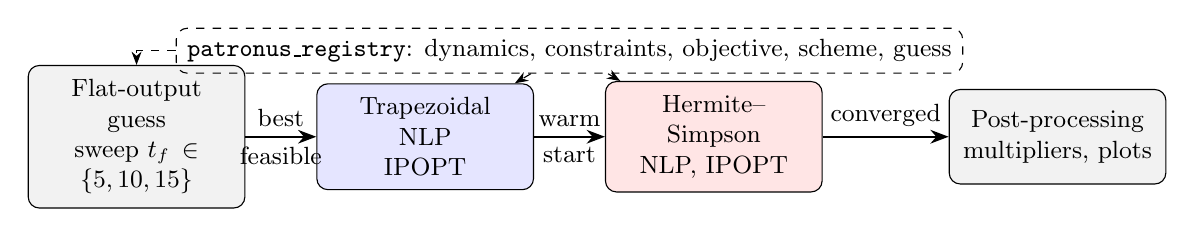
\begin{tikzpicture}[>=Stealth, font=\small, node distance=6mm and 9mm,
  box/.style={draw, rounded corners, align=center, inner sep=5pt, minimum height=12mm, text width=24mm}]
  \node[box, fill=gray!10] (g) {Flat-output guess\\ sweep $t_f \in \{5,10,15\}$};
  \node[box, fill=blue!10, right=of g] (t) {Trapezoidal NLP\\ IPOPT};
  \node[box, fill=red!10, right=of t] (hs) {Hermite--Simpson\\ NLP, IPOPT};
  \node[box, fill=gray!10, right=16mm of hs] (p) {Post-processing\\ multipliers, plots};
  \draw[->, thick] (g) -- node[above]{best} node[below]{feasible} (t);
  \draw[->, thick] (t) -- node[above]{warm} node[below]{start} (hs);
  \draw[->, thick] (hs) -- node[above]{converged} (p);
  \node[draw, dashed, rounded corners, align=center, inner sep=4pt, above=8mm of $(t)!0.5!(hs)$] (reg)
    {\code{patronus\_registry}: dynamics, constraints, objective, scheme, guess};
  \draw[->, dashed] (reg) -| (g);
  \draw[->, dashed] (reg) -- (t);
  \draw[->, dashed] (reg) -- (hs);
\end{tikzpicture}
\caption{Solution pipeline of \code{main\_vtolto\_optimizer}. Each stage builds a new NLP and
starts from the previous solution; a stage that fails to converge stops the chain.}
\label{fig:pipeline}
\end{figure}

\subsection{Scaling}
States and controls are scaled by $s = \max(|\text{min}|, |\text{max}|, 1)$ of their bounds, so IPOPT works on
$O(1)$ variables. Defects and boundary conditions are divided by the same state scales.
Box bounds are not imposed on nodes already fixed by a boundary condition: the duplicate constraint
would make the constraint Jacobian rank deficient.

\subsection{Implementation in CasADi}
\begin{itemize}
  \item \textbf{Opti stack}: the problem is written close to its mathematical form, and dual variables of
        every constraint group are available after the solve (\code{opti.dual}).
  \item \textbf{One continuous Function, mapped}: dynamics and path constraints are wrapped once as
        \code{F(x,u) -> [xdot, c, ceq, dbg]} and evaluated over the grid with \code{map}. The expression
        graph stays the size of one node, whatever $N$ is.
  \item \textbf{Exact derivatives}: algorithmic differentiation gives the sparse constraint Jacobian and
        Lagrangian Hessian, so IPOPT runs with exact second derivatives.
  \item \textbf{Registry-based architecture}: dynamics, constraint sets, objectives, schemes and guess
        generators are looked up by name in \code{patronus\_registry}. A new formulation is one line in the
        registry, not a new main script, and the cruise and take-off segments share the aircraft model.
\end{itemize}

\paragraph{Decision: CasADi.} Exact sparse first and second derivatives are what make IPOPT converge
reliably on this problem; finite differences on the nacelle Newton iterations and spline lookups
would not. CasADi also runs inside MATLAB, which keeps the existing aircraft models, and it is
the standard tool in the trajectory optimisation community.

% =====================================================================
\section{IPOPT}\label{sec:ipopt}

IPOPT solves the NLP
$\min_{\mathbf{w}} F(\mathbf{w})$ s.t. $\mathbf{c}(\mathbf{w}) = 0$, $\mathbf{w}_L \le \mathbf{w} \le \mathbf{w}_U$
by a primal--dual interior-point method (Appendix~\ref{app:ipopt}):
\begin{itemize}
  \item bounds are replaced by a logarithmic barrier with parameter $\mu \to 0$ (Figure~\ref{fig:barrier});
  \item each iteration takes a Newton step on the perturbed KKT conditions;
  \item a filter line search accepts steps that reduce either the objective or the infeasibility,
        with a feasibility restoration phase as fallback.
\end{itemize}
Settings: \code{tol} $=10^{-8}$, \code{max\_iter} $= 3000$, exact Hessian, other options at default.
\todo{report \code{mu\_strategy} and linear solver if changed}

\paragraph{Diagnostics.} An iteration callback stores $\mathbf{w}$ and $\mathbf{g}$ at every iteration.
After the solve PATRONUS reports primal and dual infeasibility, constraint violation by type,
normalised bound slack, and the multiplier of every inequality per node, from which the active
constraints are identified.

\paragraph{Decision: IPOPT.} The NLP is large, sparse and has many inequality constraints whose
active set is unknown in advance. Interior-point methods do not need to guess that active set, unlike
active-set SQP, and IPOPT exploits the exact sparse Hessian from CasADi. It is open source.

% =====================================================================
\section{Results}\label{sec:results}

\subsection{Cruise (single-point optimisation)}
The maximum-range steady cruise of the 2Wings aircraft converges with the nonlinear aerodynamic
tables and $C_P$-based power. The optimum lies at $\alpha \approx 14^\circ$, consistent with maximum
aerodynamic efficiency, with positive thrust on both groups. Only the force-balance equalities are
active; all bounds and inequalities have zero multipliers.
\todo{range, $V^*$, $\epsilon^*$, $n^*$}

\subsection{Take-off (trajectory optimisation)}
Minimum-energy take-off from hover to a trimmed hover at \SI{30}{m}, $N = 40$, trapezoidal followed by
Hermite--Simpson. Figure~\ref{fig:to} shows the converged Hermite--Simpson solution, and
Table~\ref{tab:active} the constraints active at the optimum.

\begin{figure}[h]
  \centering
  \includegraphics[width=\textwidth]{vtolto_results.pdf}
  \caption{Minimum-energy take-off: trajectory, velocities, attitude, tilt angles, propeller
  speeds, power and energy (Hermite--Simpson stage).}
  \label{fig:to}
\end{figure}

\begin{table}[h]
\centering\small
\begin{tabular}{@{}lcc@{}}
\toprule
Constraint & Multiplier & Active nodes \\
\midrule
$n_1 \le n_\text{max}$                  & 0.0634   & 8/81 \\
$x(t_f) \le \SI{2}{m}$                  & 0.0578   & 1/1 \\
$\dot n_2 \le \SI{50}{rps/s}$           & 0.0232   & 9/80 \\
$\dot n_1 \le \SI{50}{rps/s}$           & 0.0066   & 6/80 \\
$\theta \le 20^\circ$                   & 0.0040   & 1/39 \\
$\phi_2 \le 90^\circ$                   & 0.0036   & 1/41 \\
$n_2 \le n_\text{max}$                  & 0.0015   & 2/81 \\
$\dot\epsilon_2 \ge -\SI{45}{deg/s}$    & 0.0003   & 2/80 \\
\bottomrule
\end{tabular}
\caption{Active constraints at the optimum, by multiplier.}
\label{tab:active}
\end{table}

Key outcomes:
\begin{itemize}
  \item The problem converges with the full nonlinear models, from the flat guess, in both stages.
        The final stage takes about 30 IPOPT iterations (Figure~\ref{fig:ipopt}).
  \item The take-off is short, about \SI{5}{s} \todo{exact $t_f$, $E(t_f)$ and peak power}.
        In hover the rotors draw power without doing useful work, so minimising energy pushes the
        solution to climb as fast as the actuators allow.
  \item The binding limits are actuators, not aerodynamics: front-rotor speed saturation and both
        motor spin-up rates carry the largest multipliers. The rate limits are placeholders, so the
        optimum depends directly on values that still have to be confirmed.
  \item The horizontal displacement limit $x(t_f) \le \SI{2}{m}$ is active: the optimiser uses the allowed
        forward drift, tilting the thrust slightly forward.
  \item The pitch bound and $\phi_2 = 90^\circ$ are touched at single nodes only, and the tilt-rate limit
        barely, so they do not shape the solution.
\end{itemize}

\begin{figure}[h]
  \centering
  \includegraphics[width=0.75\textwidth]{ipoptMetric.pdf}
  \caption{IPOPT convergence of the Hermite--Simpson stage: reported infeasibility, constraint
  violation and normalised bound slack.}
  \label{fig:ipopt}
\end{figure}

\begin{figure}[h]
  \centering
  \includegraphics[width=0.75\textwidth]{constraint_activity.pdf}
  \caption{Constraint activity along the trajectory: constraint value and multiplier per node.}
  \label{fig:activity}
\end{figure}

\subsection{Known model limitations}
These are kept as in the cruise model and must be resolved before results are used quantitatively:
\begin{itemize}
  \item The tail pure moment uses the wing reference area and chord.
  \item In the fuselage moment the lift terms use the arm $(x_f, z_f)$ and the drag terms $(x_f, -z_f)$;
        the nacelle drag moment arms have the opposite sign to their rotors.
  \item The fuselage and tail $C_M$ tables are selected with the $C_D$ version flag, and the nacelle drag
        reuses the fuselage $C_D$ table.
  \item Fuselage arms $x_f$, $z_f$ are placeholders, and the mass needs to be confirmed against the CAD.
  \item $H_i = 0$, and the elevator is not yet in the tail model.
  \item The battery is an ideal energy store (Section~\ref{sec:battery}).
\end{itemize}

% =====================================================================
\section{Future lines of work}\label{sec:future}

\subsection{Singular arcs}
When a control enters the Hamiltonian linearly, $\partial H / \partial u = 0$ along an arc does not determine $u$:
the arc is singular, and the control follows from successive time derivatives of the switching function
(generalised Legendre--Clebsch condition). Collocation solutions on such arcs chatter, and the control-rate
regulariser hides rather than resolves this. The take-off with a minimum-time objective and bounded
controls is the natural case study: identify singular arcs from the multipliers of the converged
solution, then characterise them analytically.

\subsection{Differential flatness}
Flatness is already used for the initial guess. The next steps are: a flat parametrisation of the full
model including the thrust split, to reduce the NLP to the coefficients of the flat outputs; using it to
generate guesses for the cruise transition; and, for control allocation, mapping a flat reference
trajectory to tilts and speeds in closed form.

\subsection{Convexification (SCvx)}
Successive convexification solves a sequence of convex subproblems (SOCPs), each a linearisation of the
dynamics around the previous iterate inside a trust region, with virtual controls that keep the
subproblems feasible. It offers fast, predictable solve times and convergence guarantees, which is
what an onboard trajectory generator needs. The first prototype is a 3-DOF transition with
$\epsilon_1 = \epsilon_2$ and $n_1 = n_2$, solved first with IPOPT from a heuristic $\epsilon(t)$ guess and
then with SCvx, comparing solve time and accuracy. Locking the pairs removes the thrust split that
trims the pitching moment, so either the elevator must be added or the moment equation dropped
(point mass with $\theta$ as a control).

\subsection{Indirect methods and collocation}
The NLP multipliers of the defect constraints approximate the costates of the continuous problem.
Extracting them gives an a posteriori check of the Pontryagin conditions (costate dynamics,
transversality, constancy of $H$ for free $t_f$), and a costate guess with which to solve the
indirect problem by shooting. That would quantify the accuracy of the collocation solution and
reveal its switching structure.

\subsection{Hover-to-cruise transition}
The take-off ends in a trimmed hover and the cruise problem gives the trim at the cruise speed.
The transition connects both: free $t_f$, initial state from the take-off, terminal trim at the cruise
operating point, and the full envelope where $\alpha$ crosses stall. This is where the coarse aerodynamic
tables, the missing elevator and the nacelle drag model have the most impact, and the main
application of the SCvx work.

% =====================================================================
\appendix

\section{Model demonstration}\label{app:model}
The full derivation of \code{vtolto\_forces\_3GDL} and \code{vtolto\_dynamics\_3GDL}, including the
equivalence with Stengel's body-axis formulation, is in the companion note
\code{docs/vtolto\_dynamics.tex}. The key additional relations are summarised here.

\paragraph{Tail forces in freestream axes.}
\begin{equation}
L_t = L_t'\cos\xi - D_t'\sin\xi, \qquad D_t = D_t'\cos\xi + L_t'\sin\xi .
\end{equation}

\paragraph{Nacelle flow.}
\begin{gather}
\alpha_{n,i} = \operatorname{atan2}\!\big(V\sin\phi_i,\ v_i + V\cos\phi_i\big), \qquad
V_{n,i}^2 = V^2 + v_i^2 + 2\cos\phi_i\, v_i V, \\
D_{n,i} = C_{D,n}(\alpha_{n,i})\,\tfrac12\rho V_{n,i}^2\, A_n N_e .
\end{gather}

\paragraph{Pitching moment.} With rotor 1 at $(x_w, z_t)$ and rotor 2 at $(-x_t, z_t)$:
\begin{align}
M_{E,1} &= T_1\sin\epsilon_1\, x_w - T_1\cos\epsilon_1\, z_t, \\
M_{E,2} &= -T_2\sin\epsilon_2\, x_t - T_2\cos\epsilon_2\, z_t .
\end{align}
In hover ($\epsilon_i = 90^\circ$) pitch is trimmed by the thrust split, $T_1 x_w = T_2 x_t$.
This is the mechanism the flat guess uses and the one lost when $n_1 = n_2$ is imposed.

\paragraph{Equivalence with body axes.} The body-axis equations
$\dot u = X/m - g\sin\theta - qw$, $\dot w = Z/m + g\cos\theta + qu$ follow from \eqref{eq:eom} by
differentiating $u_b$, $w_b$, with $F_x = X\cos\theta + Z\sin\theta$ and
$F_h + mg = X\sin\theta - Z\cos\theta$. Both formulations describe the same dynamics.

\section{Optimal control}\label{app:ocp}
For $\min J = \Phi(\mathbf{x}(t_f), t_f) + \int_0^{t_f} L\,dt$ s.t.\ $\dot{\mathbf{x}} = f(\mathbf{x}, \mathbf{u})$,
$\mathbf{u} \in U$, $\boldsymbol\psi(\mathbf{x}(t_f)) = 0$:

\paragraph{Hamiltonian.}
\begin{equation}
H(\mathbf{x}, \mathbf{u}, \boldsymbol\lambda) = L(\mathbf{x}, \mathbf{u}) + \boldsymbol\lambda^\top f(\mathbf{x}, \mathbf{u}).
\end{equation}

\paragraph{Pontryagin's minimum principle.}
\begin{gather}
\dot{\boldsymbol\lambda} = -\frac{\partial H}{\partial \mathbf{x}}, \qquad
\mathbf{u}^* = \arg\min_{\mathbf{u} \in U} H(\mathbf{x}^*, \mathbf{u}, \boldsymbol\lambda), \\
\boldsymbol\lambda(t_f) = \frac{\partial \Phi}{\partial \mathbf{x}} + \boldsymbol\nu^\top \frac{\partial \boldsymbol\psi}{\partial \mathbf{x}}, \qquad
H(t_f) = -\frac{\partial \Phi}{\partial t_f} \quad (\text{free } t_f).
\end{gather}
For an autonomous problem $H$ is constant along the optimum. Path constraints add multiplier terms to
$H$ and junction conditions at the entry and exit of constrained arcs.

\paragraph{KKT conditions.} For the NLP $\min F(\mathbf{w})$ s.t.\ $\mathbf{c}(\mathbf{w}) = 0$, $\mathbf{g}(\mathbf{w}) \le 0$:
\begin{gather}
\nabla F + \nabla\mathbf{c}^\top \boldsymbol\lambda + \nabla\mathbf{g}^\top \boldsymbol\mu = 0, \qquad
\mathbf{c} = 0, \quad \mathbf{g} \le 0, \\
\boldsymbol\mu \ge 0, \qquad \mu_j\, g_j = 0 .
\end{gather}

\paragraph{Multipliers and costates.} For trapezoidal collocation the multipliers $\boldsymbol\lambda_k$
of the defects converge to the costates, $\boldsymbol\lambda(t_k) \approx \boldsymbol\lambda_k / h$
(up to sign convention). Hermite--Simpson has a similar relation but its discrete costates converge
more slowly. This is the basis of the costate-estimation check of Section~\ref{sec:future}.

\section{Transcription methods}\label{app:transcription}
\paragraph{Trapezoidal.} Integrates $\dot{\mathbf{x}}$ with the trapezoidal rule, assuming piecewise-linear
dynamics. The local error is $O(h^3)$ and the global $O(h^2)$; controls are piecewise linear. It is
equivalent to an implicit Runge--Kutta (Lobatto IIIA) method of order 2.

\paragraph{Hermite--Simpson.} The state is a cubic Hermite polynomial on each interval, matching
$\mathbf{x}_k$, $\mathbf{x}_{k+1}$, $\mathbf{f}_k$, $\mathbf{f}_{k+1}$. Its midpoint value gives the
interpolation constraint, and Simpson's rule the defect. The global error is $O(h^4)$; controls are
piecewise quadratic through the midpoint. The \emph{compressed} form substitutes the midpoint state,
so only the midpoint controls are extra variables; the \emph{separated} form keeps the midpoint state
as a variable, giving a larger but sparser NLP.

\paragraph{Choosing $N$.} With order $p$, halving $h$ reduces the error by $2^p$. For the same accuracy
Hermite--Simpson needs far fewer intervals, which compensates its extra midpoint evaluations.
\todo{mesh-refinement study: defect error vs $N$ for both schemes}

\section{CasADi}\label{app:casadi}
CasADi is a symbolic framework for algorithmic differentiation (AD) and nonlinear optimisation.
\begin{itemize}
  \item \textbf{SX and MX.} SX graphs are scalar-element expressions, fast to evaluate (used for the
        propeller maps). MX graphs are matrix-valued and allow calls to Functions, interpolants and maps
        (used for the transcription).
  \item \textbf{AD.} Forward and reverse modes give Jacobian--vector and vector--Jacobian products at a small
        multiple of the cost of one evaluation; the sparsity pattern of Jacobians and Hessians is detected
        and coloured, so full sparse derivatives are cheap.
  \item \textbf{Function and map.} A Function is a compiled expression graph; \code{map(N)} evaluates it over
        $N$ inputs without copying the graph.
  \item \textbf{Opti.} A modelling layer: variables, constraints, objective and solver options, with access to
        primal and dual solutions and to debug values on failure.
\end{itemize}

\section{IPOPT}\label{app:ipopt}
\paragraph{Barrier problem.} With slacks for the inequalities and bounds $\mathbf{w} \ge 0$,
\begin{equation}
\min_{\mathbf{w}}\ \varphi_\mu(\mathbf{w}) = F(\mathbf{w}) - \mu \sum_j \ln w_j
\quad \text{s.t.} \quad \mathbf{c}(\mathbf{w}) = 0 .
\end{equation}
\paragraph{Primal--dual system.} With $\mathbf{z}$ the bound multipliers, the perturbed KKT conditions are
\begin{equation}
\nabla F + \nabla\mathbf{c}^\top\boldsymbol\lambda - \mathbf{z} = 0, \qquad
\mathbf{c} = 0, \qquad W Z \mathbf{e} = \mu\mathbf{e},
\end{equation}
and each iteration solves the Newton system
\begin{equation}
\begin{bmatrix} \nabla^2_{ww}\mathcal{L} + \Sigma & \nabla\mathbf{c}^\top \\ \nabla\mathbf{c} & 0 \end{bmatrix}
\begin{bmatrix} \Delta\mathbf{w} \\ \Delta\boldsymbol\lambda \end{bmatrix}
= - \begin{bmatrix} \nabla\varphi_\mu + \nabla\mathbf{c}^\top\boldsymbol\lambda \\ \mathbf{c} \end{bmatrix},
\qquad \Sigma = W^{-1} Z,
\end{equation}
with inertia correction when the reduced Hessian is not positive definite.

\begin{figure}[h]
\centering
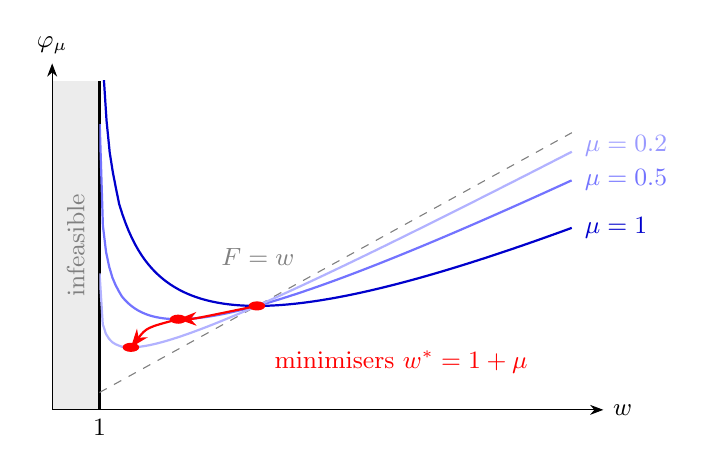
\begin{tikzpicture}[>=Stealth, font=\small, xscale=2.0, yscale=1.1]
  \fill[gray!15] (0.7,0.8) rectangle (1,4.6);
  \node[rotate=90, gray] at (0.85,2.7) {infeasible};
  \draw[->] (0.7,0.8) -- (4.2,0.8) node[right]{$w$};
  \draw[->] (0.7,0.8) -- (0.7,4.8) node[above]{$\varphi_\mu$};
  \draw[thick] (1,0.8) -- (1,4.6);
  \node[below] at (1,0.8) {$1$};
  \begin{scope}
    \clip (1,0.8) rectangle (4.2,4.6);
    \draw[gray, dashed, domain=1:4] plot (\x, \x);
    \draw[thick, blue!80!black, domain=1.005:4, samples=150] plot (\x, {\x - 1.0*ln(\x-1)});
    \draw[thick, blue!55, domain=1.002:4, samples=150] plot (\x, {\x - 0.5*ln(\x-1)});
    \draw[thick, blue!30, domain=1.001:4, samples=150] plot (\x, {\x - 0.2*ln(\x-1)});
  \end{scope}
  \fill[red] (2,2) circle (1.5pt);
  \fill[red] (1.5,1.8466) circle (1.5pt);
  \fill[red] (1.2,1.5219) circle (1.5pt);
  \draw[red, ->, thick] (2,2) .. controls (1.6,1.85) .. (1.5,1.8466);
  \draw[red, ->, thick] (1.5,1.8466) .. controls (1.3,1.75) .. (1.2,1.5219);
  \node[blue!80!black, anchor=west] at (4.02,2.90) {$\mu = 1$};
  \node[blue!55, anchor=west] at (4.02,3.45) {$\mu = 0.5$};
  \node[blue!40, anchor=west] at (4.02,3.85) {$\mu = 0.2$};
  \node[gray, anchor=south east] at (2.3,2.35) {$F = w$};
  \node[red, align=left, anchor=west] at (2.05,1.35) {minimisers $w^* = 1 + \mu$};
\end{tikzpicture}
\caption{Log-barrier for $\min w$ s.t.\ $w \ge 1$:
$\varphi_\mu(w) = w - \mu\ln(w-1)$. Each barrier problem has an interior minimiser
$w^*(\mu) = 1 + \mu$; as $\mu \to 0$ these points (the central path) approach the constrained
optimum $w = 1$ from inside the feasible set, which is how IPOPT treats every bound and inequality.}
\label{fig:barrier}
\end{figure}

\paragraph{Globalisation.} A fraction-to-the-boundary rule keeps $\mathbf{w} > 0$, and a filter line search
accepts a trial point if it sufficiently reduces $\varphi_\mu$ or $\|\mathbf{c}\|$. If no acceptable step
exists, a restoration phase minimises the infeasibility. $\mu$ decreases when the barrier problem is
solved to a tolerance proportional to $\mu$.

\section{Differential flatness}\label{app:flatness}
A system $\dot{\mathbf{x}} = f(\mathbf{x}, \mathbf{u})$ is differentially flat if there exist outputs
$\mathbf{y} = h(\mathbf{x}, \mathbf{u}, \dot{\mathbf{u}}, \dots)$, with $\dim\mathbf{y} = \dim\mathbf{u}$, such that
\begin{equation}
\mathbf{x} = \Psi_x(\mathbf{y}, \dot{\mathbf{y}}, \dots, \mathbf{y}^{(r)}), \qquad
\mathbf{u} = \Psi_u(\mathbf{y}, \dot{\mathbf{y}}, \dots, \mathbf{y}^{(r+1)}) .
\end{equation}
Any sufficiently smooth $\mathbf{y}(t)$ then defines a trajectory that satisfies the dynamics exactly,
so trajectory planning reduces to choosing $\mathbf{y}(t)$ and checking constraints.

For the take-off, with $H = 0$, no nacelle drag and $\epsilon_1 = \epsilon_2 = \epsilon$, the outputs
$\mathbf{y} = (x, h, \theta)$ determine $v_x, v_h, q$ by differentiation, the thrust vector from the force
balance, $\epsilon$ from its direction, and $T_1$, $T_2$ from the force and moment balances. The model has
four controls and three outputs; the extra freedom is removed by $\epsilon_1 = \epsilon_2$. Each output is
a quintic in $\tau = t/t_f$, the lowest degree that meets position, velocity and acceleration at both
ends.

\section{Convex optimisation: brief literature review}\label{app:convex}
\begin{itemize}
  \item \textbf{Foundations.} Boyd and Vandenberghe~\cite{boyd2004} establish convex sets and functions,
        duality and the standard conic forms (LP, QP, SOCP, SDP) solved by interior-point methods in
        polynomial time with certificates of optimality.
  \item \textbf{Lossless convexification.} Açıkmeşe and Ploen~\cite{acikmese2007} showed that the
        non-convex thrust lower bound of powered descent can be relaxed into a convex constraint without
        changing the optimum, via the maximum principle. Later work generalised the conditions under which
        the relaxation is exact.
  \item \textbf{Successive convexification.} Mao, Szmuk and Açıkmeşe~\cite{mao2016} proposed SCvx, which
        handles general non-convex dynamics by successive linearisation, trust regions and virtual controls,
        with convergence guarantees. Szmuk and co-workers applied it to quadrotor and 6-DOF powered-descent
        trajectories in real time.
  \item \textbf{Survey.} Malyuta et al.~\cite{malyuta2022} review convex optimisation for trajectory
        generation, comparing lossless convexification, SCvx and penalised trust-region methods.
  \item \textbf{Relevance.} The tilt-rotor transition has non-convex aerodynamics and coupled thrust
        vectoring, so lossless convexification alone does not apply; SCvx is the candidate, with the
        IPOPT solution of this report as the reference.
\end{itemize}

\begin{thebibliography}{9}
\bibitem{betts2010} J.~T. Betts, \emph{Practical Methods for Optimal Control and Estimation Using Nonlinear Programming}, 2nd ed., SIAM, 2010.
\bibitem{kelly2017} M.~Kelly, ``An introduction to trajectory optimization: how to do your own direct collocation,'' \emph{SIAM Review}, 59(4), 2017.
\bibitem{andersson2019} J.~A.~E. Andersson, J.~Gillis, G.~Horn, J.~B. Rawlings and M.~Diehl, ``CasADi: a software framework for nonlinear optimization and optimal control,'' \emph{Mathematical Programming Computation}, 11, 2019.
\bibitem{wachter2006} A.~Wächter and L.~T. Biegler, ``On the implementation of an interior-point filter line-search algorithm for large-scale nonlinear programming,'' \emph{Mathematical Programming}, 106, 2006.
\bibitem{fliess1995} M.~Fliess, J.~Lévine, P.~Martin and P.~Rouchon, ``Flatness and defect of non-linear systems,'' \emph{International Journal of Control}, 61(6), 1995.
\bibitem{tremblay2007} O.~Tremblay, L.-A. Dessaint and A.-I. Dekkiche, ``A generic battery model for the dynamic simulation of hybrid electric vehicles,'' IEEE Vehicle Power and Propulsion Conference, 2007.
\bibitem{boyd2004} S.~Boyd and L.~Vandenberghe, \emph{Convex Optimization}, Cambridge University Press, 2004.
\bibitem{acikmese2007} B.~Açıkmeşe and S.~R. Ploen, ``Convex programming approach to powered descent guidance for Mars landing,'' \emph{Journal of Guidance, Control, and Dynamics}, 30(5), 2007.
\bibitem{mao2016} Y.~Mao, M.~Szmuk and B.~Açıkmeşe, ``Successive convexification of non-convex optimal control problems and its convergence properties,'' IEEE Conference on Decision and Control, 2016.
\bibitem{malyuta2022} D.~Malyuta, T.~P. Reynolds, M.~Szmuk, T.~Lew, R.~Bonalli, M.~Pavone and B.~Açıkmeşe, ``Convex optimization for trajectory generation,'' \emph{IEEE Control Systems Magazine}, 42(5), 2022.
\end{thebibliography}

\end{document}
